\subsubsection{GUI}
Programmet QT blev anvendt til at designe og implementere brugergrænsefladen. Udfordringerne i brugen af dette værktøj bestod primært i, at kendskabet til programmet ikke var særligt stort. \\

Da QT selv skaber klasserne og metoderne er det svært at beskrive disse på forhånd. Derfor blev det besluttet at klasserne først skulle udarbejdes efter at brugergrænsefladen var designet.

Det endelige klassediagram der blev udarbejdet kan ses illustreret på figur \ref{kd}. Dette klassediagram indeholder 5 forskellige klasser.

\begin{figure}[H]
	\centerline{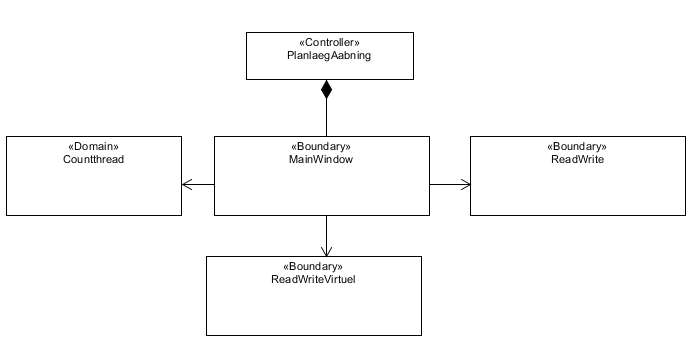
\includegraphics[scale=0.6]{tex/Design/GUI/Fotos/Tom_klassediagram_GUI}}
	\caption{Klasserne indsættes i et klassediagram}
	\label{kd}
\end{figure}


For at holde styr på den indtastede og den resterende tid er der blev oprettet en Count klasse. Denne count klasse er implementeret som en domainklasse da det er her den resterende tid for vinåbningen gemmes. Det er denne klasse som skal sørge for at tiden tælles ned når den startes. Illustrationen af countklassen kan ses på figur \ref{CT_CD}.

\begin{figure}[H]
	\centerline{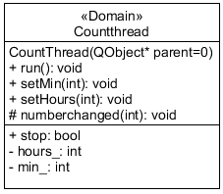
\includegraphics[scale=1]{tex/Design/GUI/Fotos/CountThread}}
	\caption{CountThread klasse illustreret}
	\label{CT_CD}
\end{figure}

Der er 3 klasser for brugergrænsefladen. Der er en klasse for MainWindow, hvor alle funktionerne for den grafiske del af brugergrænsefladen er defineret.  Det er her alle trykknap funktionerne er defineret. Klassen ses illustreret på figur \ref{MW_CD}. 

\begin{figure}[H]
	\centerline{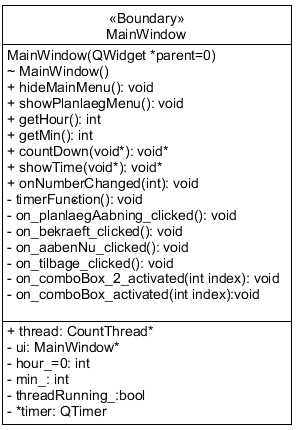
\includegraphics[scale=1]{tex/Design/GUI/Fotos/MainWindow}}
	\caption{MainWindow klasse illustreret}
	\label{MW_CD}
\end{figure}

Der er yderligere blevet implementeret en klasse til at sende og modtage kommandoer fra PSoC. Dette er gjort, fordi at det skal være muligt at kunne teste denne klasse for sig. Yderligere giver fås et større overblik hvis funktionerne er fordelt over de rigtige klasser. Dette vil medføre til at systemet har en lav kobling, hvilket fører til at man let kan ændre, tilføje og rette i koden. Klassen ReadWrite indholder 2 funktioner. En til at læse fra PSoC og en til at skrive til den.

For at se hele klasse diagrammet med alle metoder henvises der til bilag\footnote{Se GUI\_CD}.

Brugergrænsefladen er state styret. Derfor har det været nødvendigt at lave et statemachine diagram for brugergrænsefladen. Statemachinen ses på figur \ref{sm}.\\

\begin{figure}[H]
	\centerline{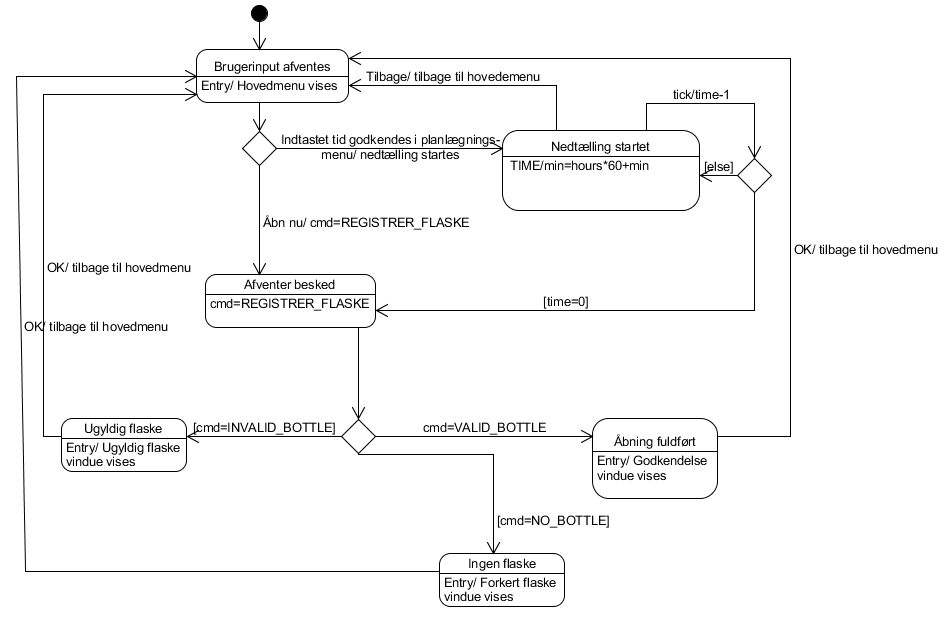
\includegraphics[scale=1]{tex/Design/GUI/Fotos/sm}}
	\caption{statemachine}
	\label{sm}
\end{figure}

I følgende afsnit vil de forskellige states som er illustreret på figur \ref{sm} blive beskrevet.

\textbf{Brugerinput afventes}\\
Når systemet starter op vil brugeren befinde sig i denne state. Her vil brugergrænsefladens hovedmenu vises. Brugeren vil herfra have muligheden om enten at trykke på "Åbn nu" eller at planlægge åbningen ved at trykke på "Planlæg åbning".\\

\textbf{Nedtælling startet}\\
Hvis brugeren vælger vælger en tid i planlægningsmenuen og trykker på bekræft vil denne state aktiveres. Her vil den indtastede tid konverteres til minutter og nedtællingen fra den konverterede tid startes. Når nedtællingen når 0 brydes der ud af denne state. Imens systemet er i denne state er det muligt for brugeren at navigere i systemet og gå tilbage til hovedmenuen ved at trykke tilbage på brugergrænsefladen.\\

\textbf{Afventer besked}\\
Når brugeren vælger menupunktet "Åbn nu" eller tiden tælles ned til 0 sættes cmd til at være REGISTRER\_FLASKE og denne state aktiveres. I denne state ventes der på svar fra PSoC. Systemet kan her modtage 3 forskellige cmd's: INVALID\_BOTTLE, VALID\_BOTTLE og NO\_BOTTLE. Den besked som systemet modtager vil være den der sættes i cmd.\\

\textbf{Ugyldig flaske}\\
Hvis cmd blev sat til INVALID\_BOTTLE aktiveres denne state. Her modtager brugeren en besked om at flasken er invalid.\\

\textbf{Ingen flaske}\\
Hvis cmd blev sat til NO\_BOTTLE aktiveres denne state. Her modtager brugeren en besked om at en vinflaske skal indsættes.
\\

\textbf{Åbning fuldført}\\
Hvis cmd blev sat til VALID\_BOTTLE aktiveres denne state. Her modtager brugeren en besked om at en vinflasken er godkendt, og at åbningen påbegyndes.\\


De tre sidste states fører brugeren tilbage til hovedmenuen ved at brugeren trykker OK på vinduet.
